%!TEX root = Slic3r-Manual.tex
\section{Mode Simple} % (fold)
\label{sec:simple_mode}
\index{simple mode}
\index{mode simple}

Slic3r a deux modes de fonctionnement, Simple et Expert. Ceux-ci peuvent être choisis à partir de la fenêtre \texttt{Preferénces} (qui se trouve dans le menu  \texttt{File} (fichier) ).

\begin{figure}[ht]
\centering
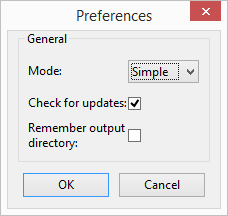
\includegraphics[width=0.3\textwidth]{simple_mode/preferences_general.png}
\caption{Preférences.}
\label{fig:preferences_general}
\end{figure}

Le mode simple offre une gamme réduite de paramètres, suffisament pour que le débutant puisse commencer. Le mode expert donne plus de contrôle sur la manière dont Slic3r produit le G-code, celui-ci sera examiné plus tard.

\subsection{Paramètres d'Impression}
\index{Print Settings}
\index{paramètres d'impression}

L'onglet \texttt{Print Settings} (paramètres d'impression) 
offre la possibilité de modifier les paramètres liés à l'impression réelle. Alors que les autres onglets sont modifiées moins souvent, les paramètres de cet onglet seront modifiés régulièrement, éventuellement pour chaque modèle imprimé.

\begin{figure}[ht]
\centering
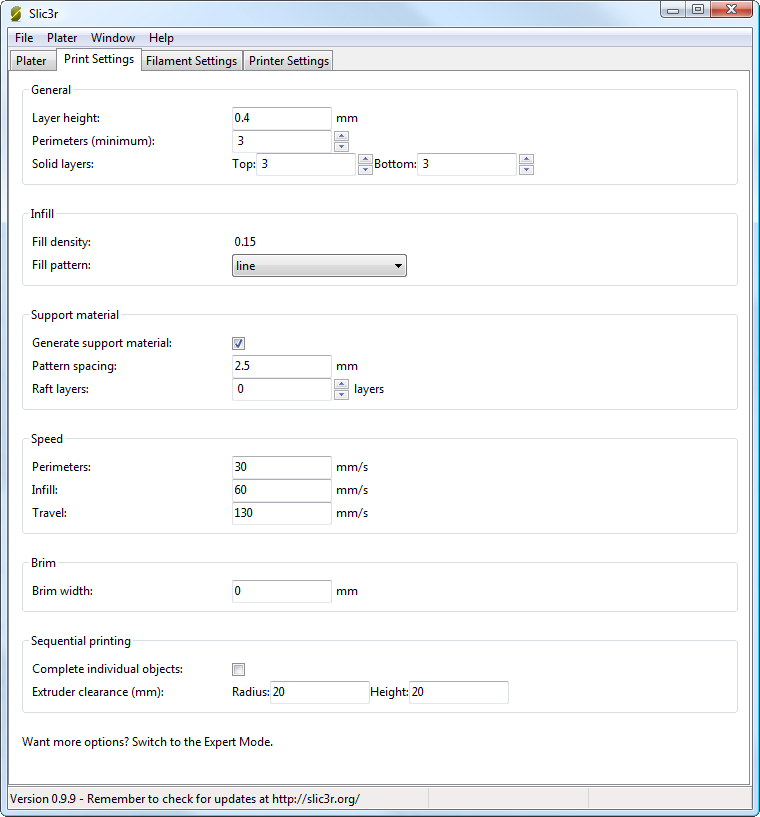
\includegraphics[width=\textwidth]{simple_mode/simple_mode_print_settings.png}
\caption{Mode Simple: Paramètres d'impression.}
\label{fig:simple_mode_print_settings}
\end{figure}

\paragraph{Général.} % (fold)
\label{par:simple_general}
\index{Print Settings!Layer height}
\index{Paramètres d'impression!Epaisseur de couche}

\texttt{Layer height} (épaisseur de couche) définit le déplacement sur l'axe vertical avant l'extrusion d'une nouvelle couche.  Il y a plusieurs facteurs qui influentsur la hauteur que la couche doit avoir:
\begin{itemize}
	\item \textbf{Résolution Désirée}  - Une faible hauteur de couche devrait conduire à des impressions avec des nervures ou des bandes moins visibles, comme chaque couche est plus petite. L'esthétique joue ici un rôle, mais aussi le type de modèle, par exemple, une pièce mécanique peut ne pas avoir besoin d'une telle finition haute résolution, alors qu'une pièce de présentation peut en avoir besoin.
	\item \textbf{Vitesse d'impression}  - Les couches plus fines produiront des impression lisses, mais chaque impression prendra plus de temps, tout simplement parce que l'extrudeuse doit tracer le motif plusieurs fois. Un des buts plus tard sera de trouver un équilibre entre la hauteur de couche, la vitesse de l'imprimante, et la qualité de l'impression qui en résulte.
\end{itemize}
\index{Print Settings!Perimeters}
\index{Paramètres d'impression!Périmètres}
\texttt{Perimeters} (Périmetres) définit le nombre minimum de coquilles verticales (c'est à dire les murs) que l'impression aura. À moins que le modèle ne nécessite qu'un seul mur, il est généralement recommandé d'avoir un minimum de deux périmètres car cela donne l'assurance que si une partie du périmètre ne s'imprime pas correctement alors le second périmètre permettra le de couvrir.

\index{Print Settings!Solid layers}
\index{Paramètres d'impression!Couches pleines}
Les couches supérieure et inférieure qui prennent en sandwich le modèle sont remplis de motifs de \texttt{Solid layers} (couches pleines). Pour les couches inférieures (bottom) le facteur important à prendre en compte est la façon dont la surface aura l'air s'il y avait une anomalie, lors de l'impression de la première couche, c'est pour cette raison, qu'il est recommandé d'avoir au moins deux couches inférieures.

Une prise en compte similaire est nécessaire pour les couches supérieures (top). Parce que les couches intermédiaires sont susceptibles d'être rempli d'un motif fixé à moins de 100\% , les couches de revêtement devront combler ce motif et cela peut nécessiter plus d'un passage pour le couvrir complètement.

\begin{figure}[H]
\centering
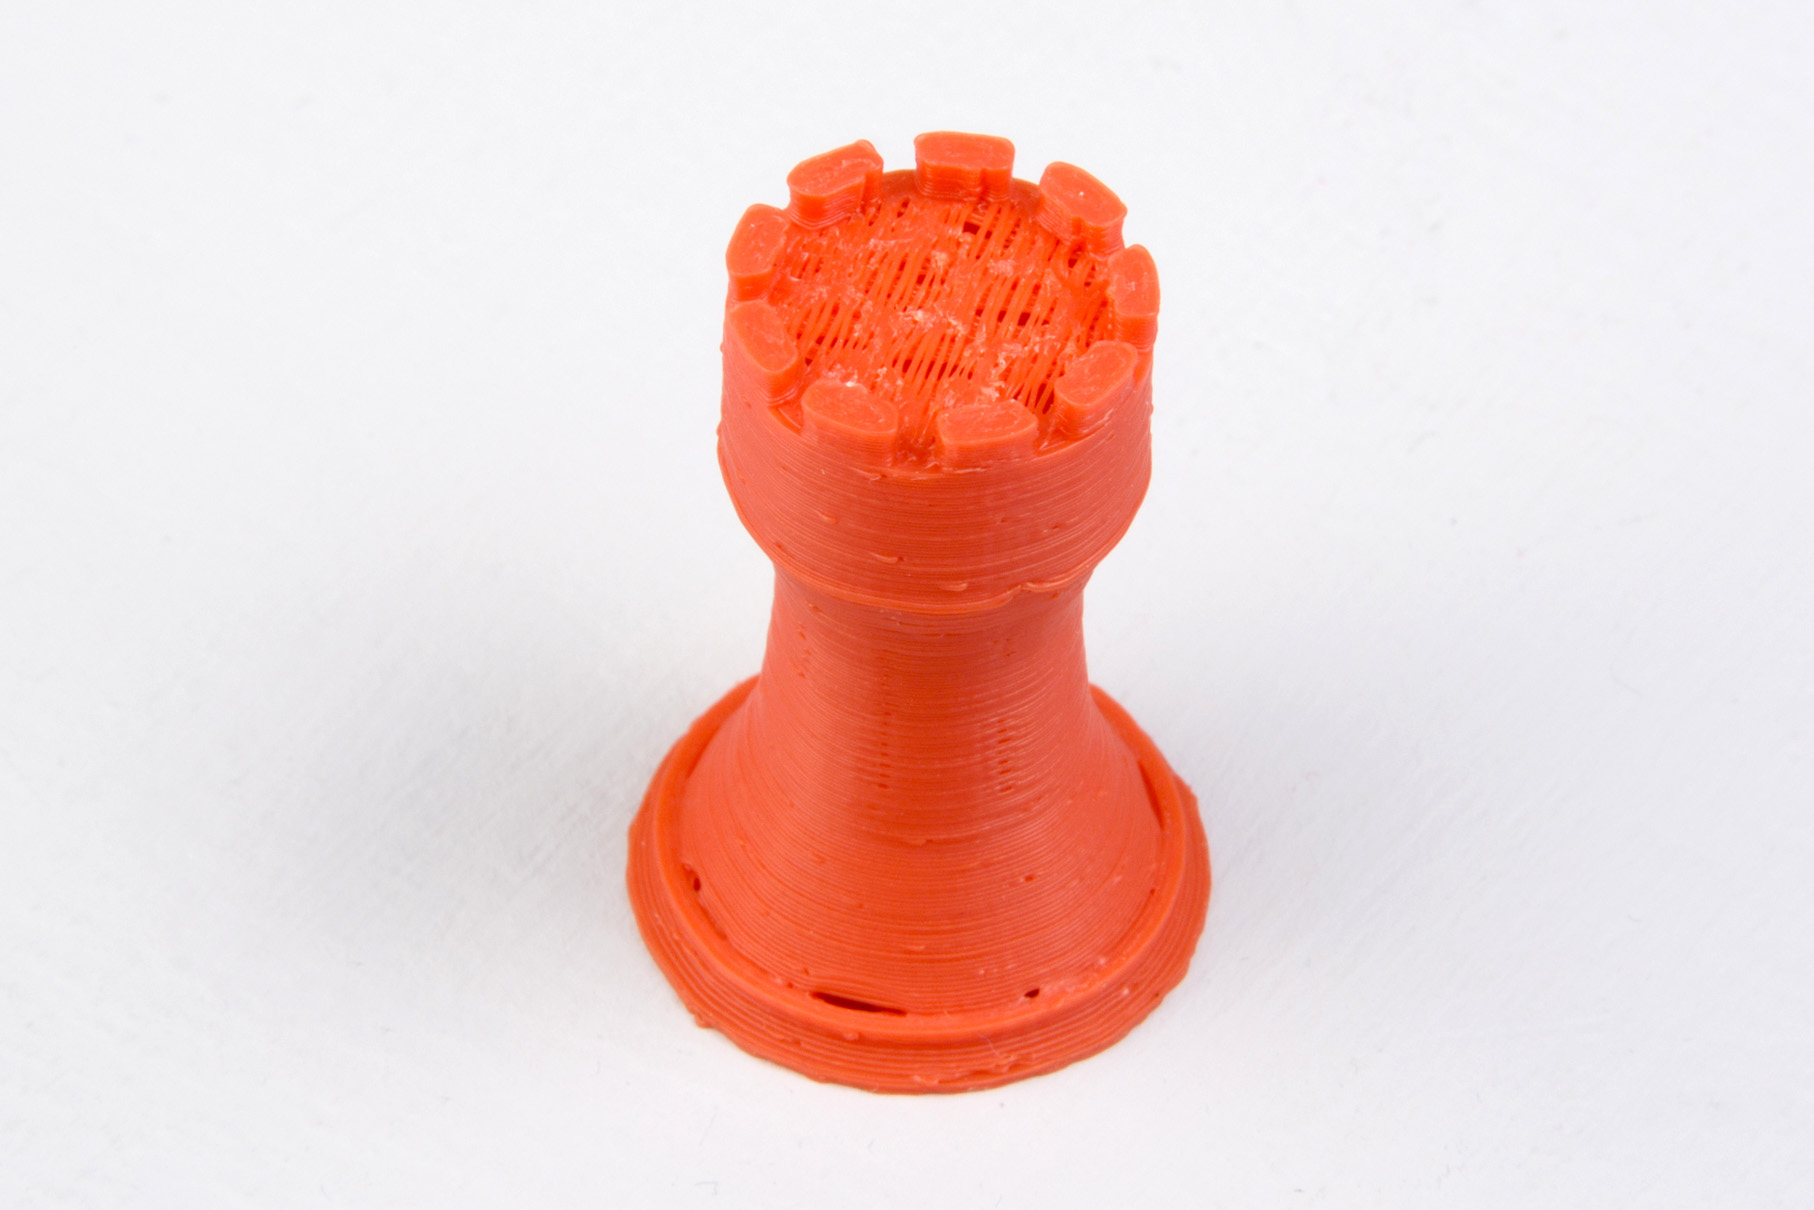
\includegraphics[keepaspectratio=true,width=0.75\textwidth]{simple_mode/bad_top_infill.jpg}
\caption{Un exemple de couches supérieures insuffisantes.}
\label{fig:bad_top_infill}
\end{figure}

Une autre astuce à considérer: Régler la couche pleine supérieure (top solid layer) à zéro, et régler le remplissage également à zéro, produira un récipient , idéal pour transformer les modèles en vases\footnote{http://slic3r.org/blog/tip-printing-vases} par exemple. Ici la modification des paramètres peuvent être utilisés dans Slic3r pour générer différents types de impressions, et pas seulement pour contrôler la précision de surface.

\begin{figure}[H]
\centering
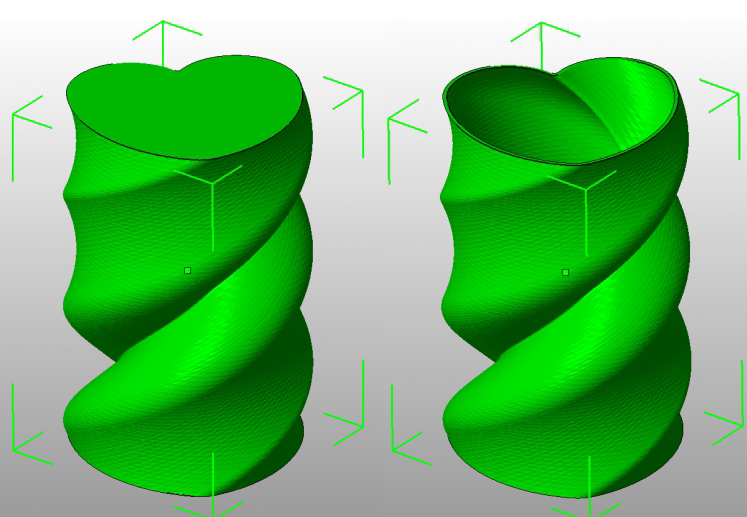
\includegraphics[keepaspectratio=true,width=0.75\textwidth]{simple_mode/solid_layers_vases.png}
\caption{Création d'un vase à partir d'un modèle solide.}
\label{fig:solid_layers_vases}
\end{figure}

% paragraph general (end)

\paragraph{Remplissage. (Infill)} % (fold)
\label{par:simple_infill}
\index{Print Settings!Infill}
\index{Paramètres d'impression!Remplissage}
\index{Print Settings!Infill!Fill density}
\index{paramètres d'impression!Densitée de remplissage}
\texttt{Fill density} (Densité de remplissage) est définie sur une échelle comprise entre 0 et 1, où 1 est de 100\% et 0,4 serait 40\%. Pour la majorité des cas, remplir la pièce à 100\% n'a pas d'intérêt, ce serait un gaspillage de matériel et prendrait beaucoup de temps. Au lieu de cela, la plupart des modèles peuvent être remplis avec moins de matière, qui sera ensuite pris en sandwich entre les couches remplies à 100\% (voir \texttt{Solid layers} au dessus).

Une valeur de densité de 0,4 est suffisant pour donner à la quasi-totalité des modèles une bonne résistance mécanique. Une valeur de 0,2 est généralement le minimum requis pour soutenir des plafonds plats.

\index{Print Settings!Infill!Fill pattern}
Slic3r offre plusieurs motifs de remplissage qui seront examinés plus en détail dans la section \ref{sec:infill_patterns_and_density} - Motifs et densitée de remplissage.  Choisir un \texttt{Fill pattern} (motif de remplissage) dépendra du type de modèle, la résistance souhaitée de la structure , la vitesse d'impression, et des goûts personnels. Les modes de remplissage plus exotiques sont généralement trop lent et inutilement complexe pour la plupart des cas d'utilisation, et donc la plupart du temps, le motif de remplissage est soit \texttt{rectilinear} (rectiligne), \texttt{line} (ligne), or \texttt{honeycomb} (nid d'abeille).  Honeycomb offre le plus résistance, mais est plus lent que les deux rectilinear ou line.

% paragraph infill (end)

\paragraph{Support. (Support material)} % (fold)
\label{par:simple_support_material}
\index{Print Settings!Support material}
\index{Paramètres d'impression!Support}
\index{Print Settings!Support material!Generate support material}
\index{Paramètres d'impression!Support!Générer le support}
\index{Print Settings!Support material!Pattern spacing}
\index{Paramètres d'impression!Support!Espacement du motif}
Imprimer un modèle de bas en haut, avec une imprimante FDM, signifie que les saillies importantes seront imprimées dans le vide, pruduisant des affaissement ou un mauvais résultat.  Obter pour un support (\texttt{Generate support material}) ajoutera des structures supplémentaires dans le modèle qui seront construites pour soutenir la partie en surplomb. Le paramètre \texttt{Pattern spacing} (espacement du motif) détermine la densité du support qui est imprimé.

\begin{figure}[H]
\centering
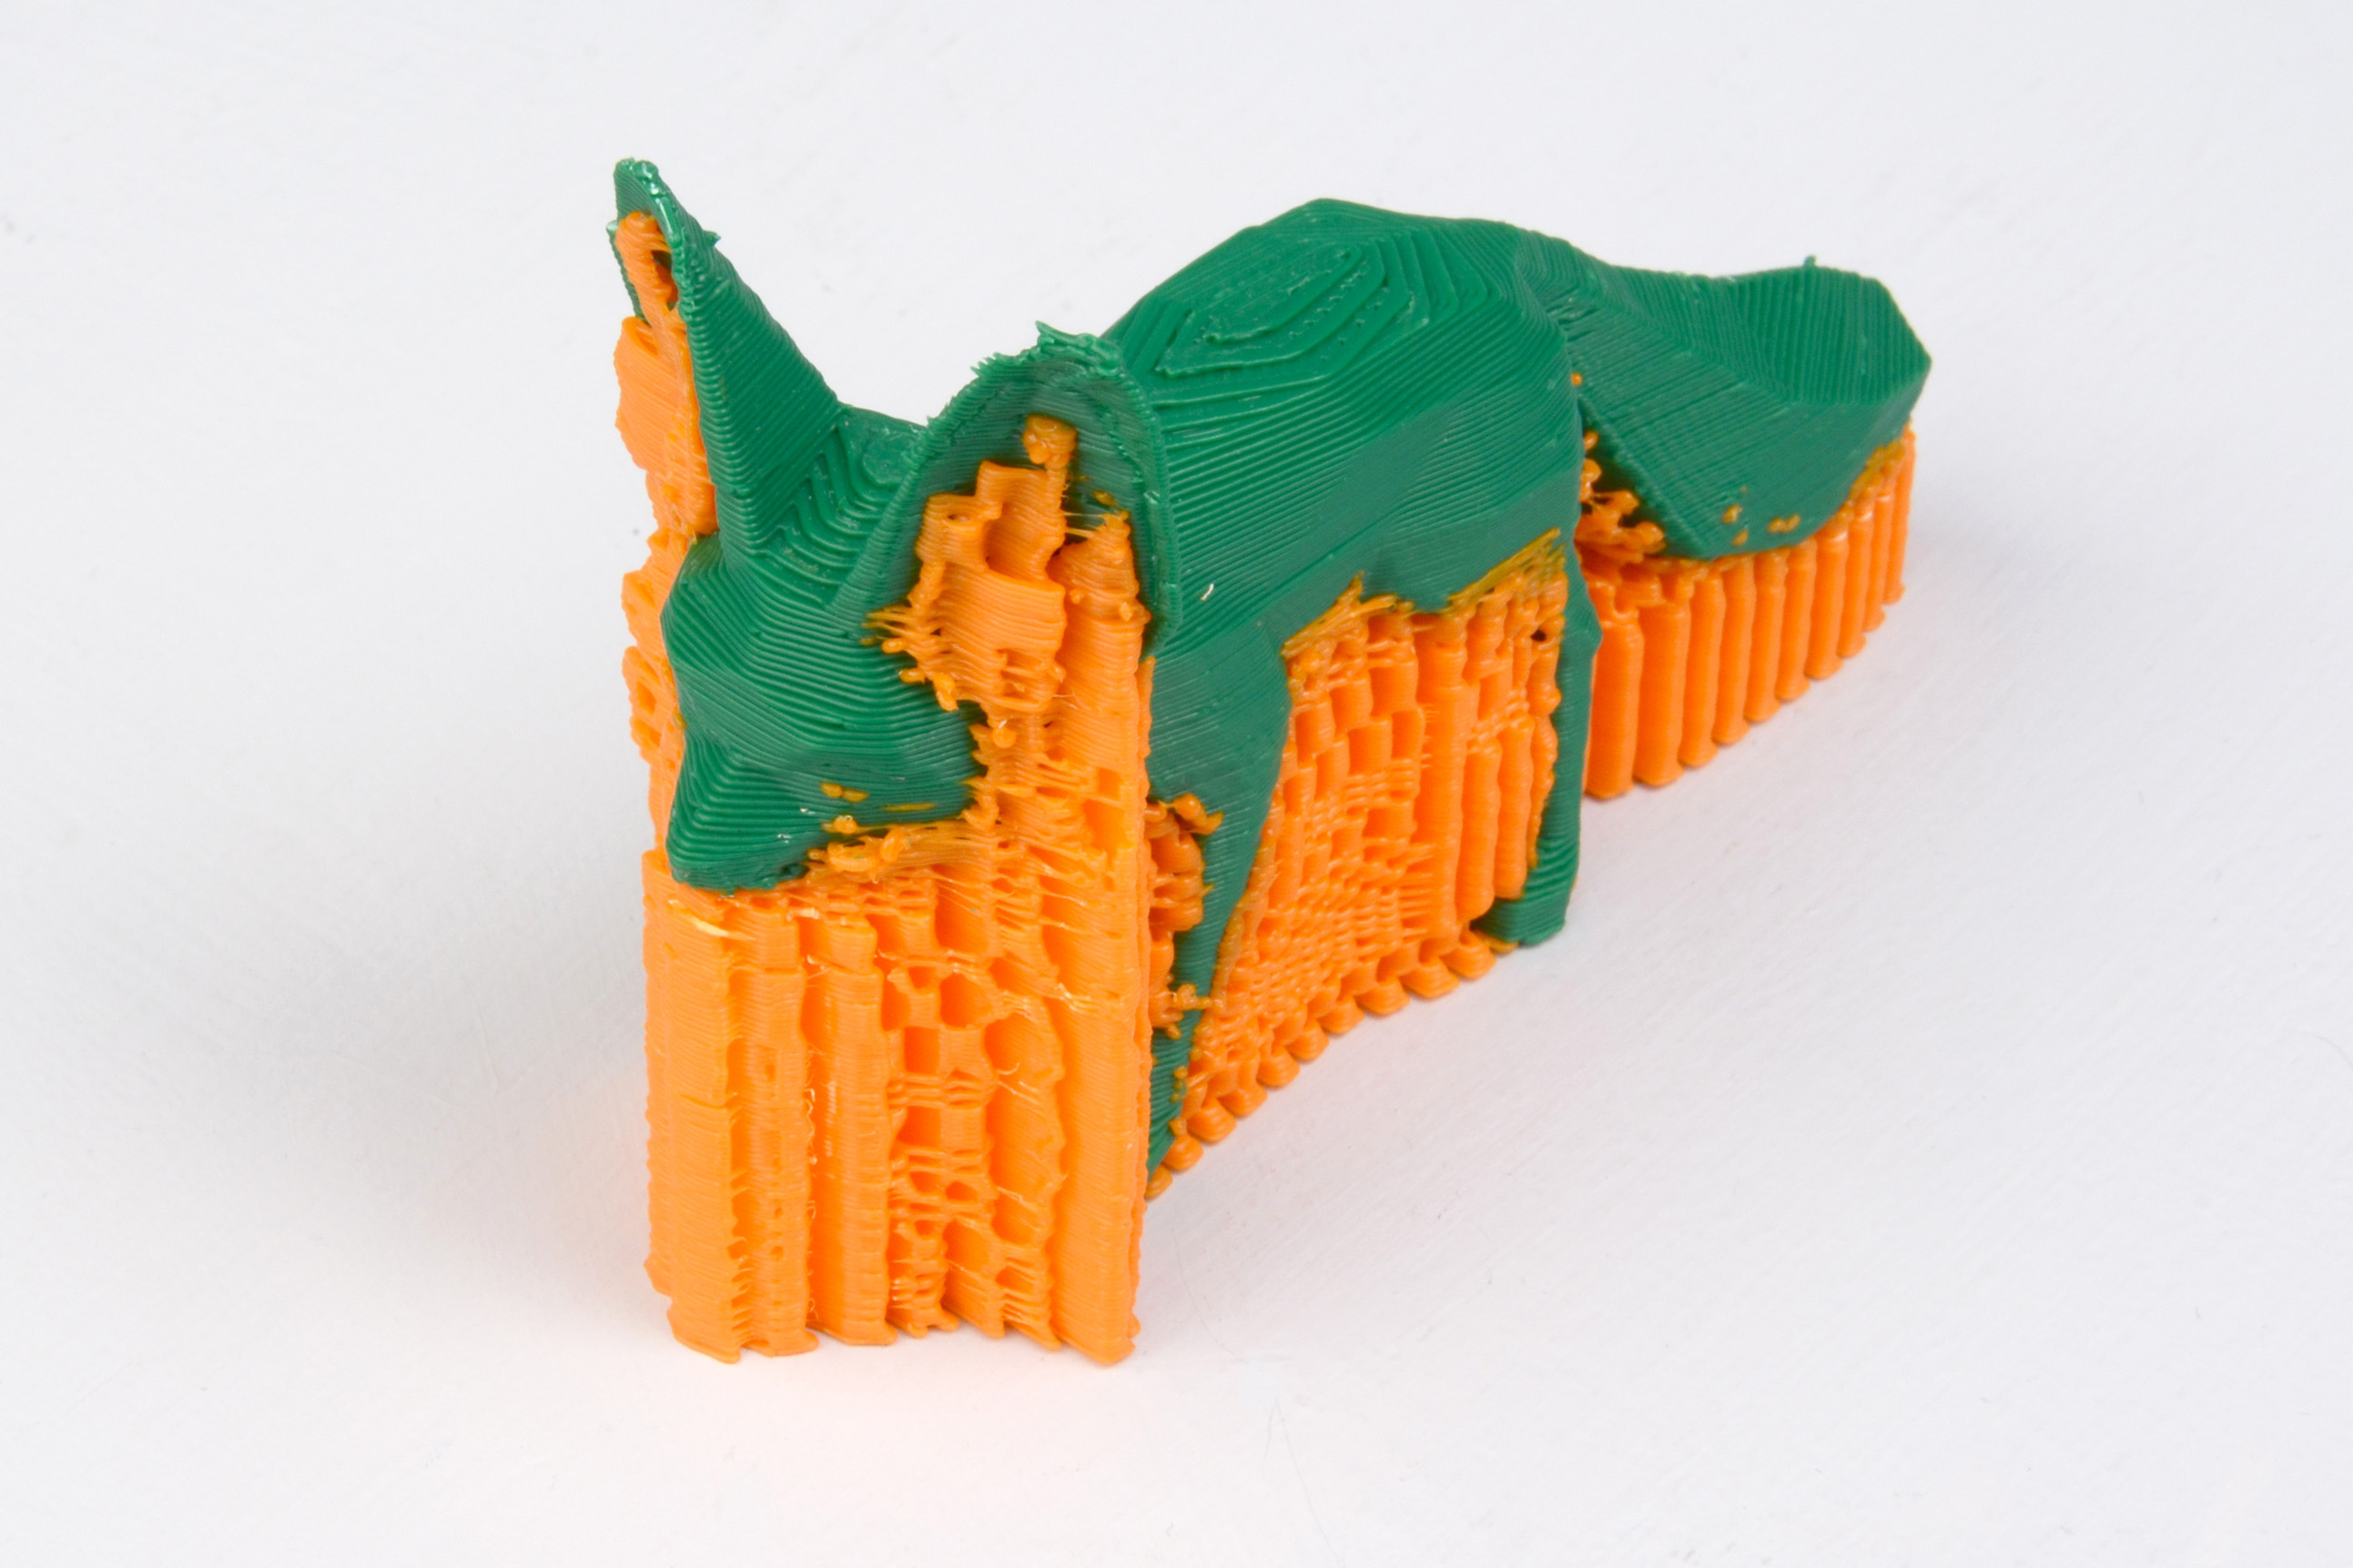
\includegraphics[keepaspectratio=true,width=0.75\textwidth]{simple_mode/support_example.jpg}
\caption{Un exemple d'un objet imprimé avec un support.}
\label{fig:support_example}
\end{figure}

Astuce: Il est parfois utile d'envisager de modifier l'orientation du modèle afin de réduire éventuellement les surplombs.

\index{Print Settings!Support material!Raft layers}
\index{Paramètres d'impression!Support!Radier}
\texttt{Raft layers} (radier) va ajouter des couches supplémentaires sous le modèle et découle depuis les débuts de l'impression 3D. Il peut vous aider à imprimer sans lit chauffé, ou lorsque le lit n'est pas très plat, mais il n'est généralement pas nécessaire et n'est pas recommandé. Le radier nécessite en outre un post-traitement pour le supprimer.
% paragraph support_material (end)

\paragraph{Vitesse. (Speed)} % (fold)
\label{par:simple_speed}
\index{Print Settings!Speed}
En mode simple, il n'y a que trois réglages de vitesse à configurer:
\index{Print Settings!Speed!Perimeters}
\index{Paramètres d'impression!Périmètres}
\index{Print Settings!Speed!Infill}
\index{Paramètres d'impression!Vitesse!Remplissage}
\index{Print Settings!Speed!Travel}
\index{Paramètres d'impression!Vitesse!Déplacement}
\begin{itemize}
	\item \texttt{Perimeters} (Perimeters) - Le contour du modèle peut bénéficier d'une vitesse d'impression légèrement plus lente de sorte que la peau extérieure de l'impression ait moins de défauts.
	\item \texttt{Remplissage} (Infill) - Comme le remplissage est caché il peut être extrudé un peu plus vite. Prenez bien soin de ne pas aller trop vite, car plus la vitesse est élevée, et plus les extrusions sont minces, et cela peut affecter la façon dont se fait la liaison entre les extrusions.
	\item \texttt{Déplacement} (Travel) - Le saut entre la fin d'une extrusion et la suivante doivent généralement être effectuées aussi rapidement que l'imprimante le permet , afin de minimiser les dégâts causés par suintement de matériau depuis la buse.
\end{itemize}
% paragraph speed (end)

\paragraph{Bordure. (Brim)} % (fold)
\label{par:simple_brim}
\index{Print Settings!Brim}
\index{Paramètres d'impression!Bordure}
\index{Print Settings!Brim!Brim width}
\index{Paramètres d'impression!Bordure!Largeur de bordure}
\texttt{Brim width} (largeur de bordure) est utilisé pour ajouter plus de périmètres à la première couche, en tant base supplémentaire, afin de fournir une plus grande surface pour que l'impression colle au lit , afin de réduire les déformation (voir §\ref{sec:the_important_first_layer}). Le bord est ensuite découpée une fois que l'impression est terminée et retirée du lit.

\begin{figure}[H]
\centering
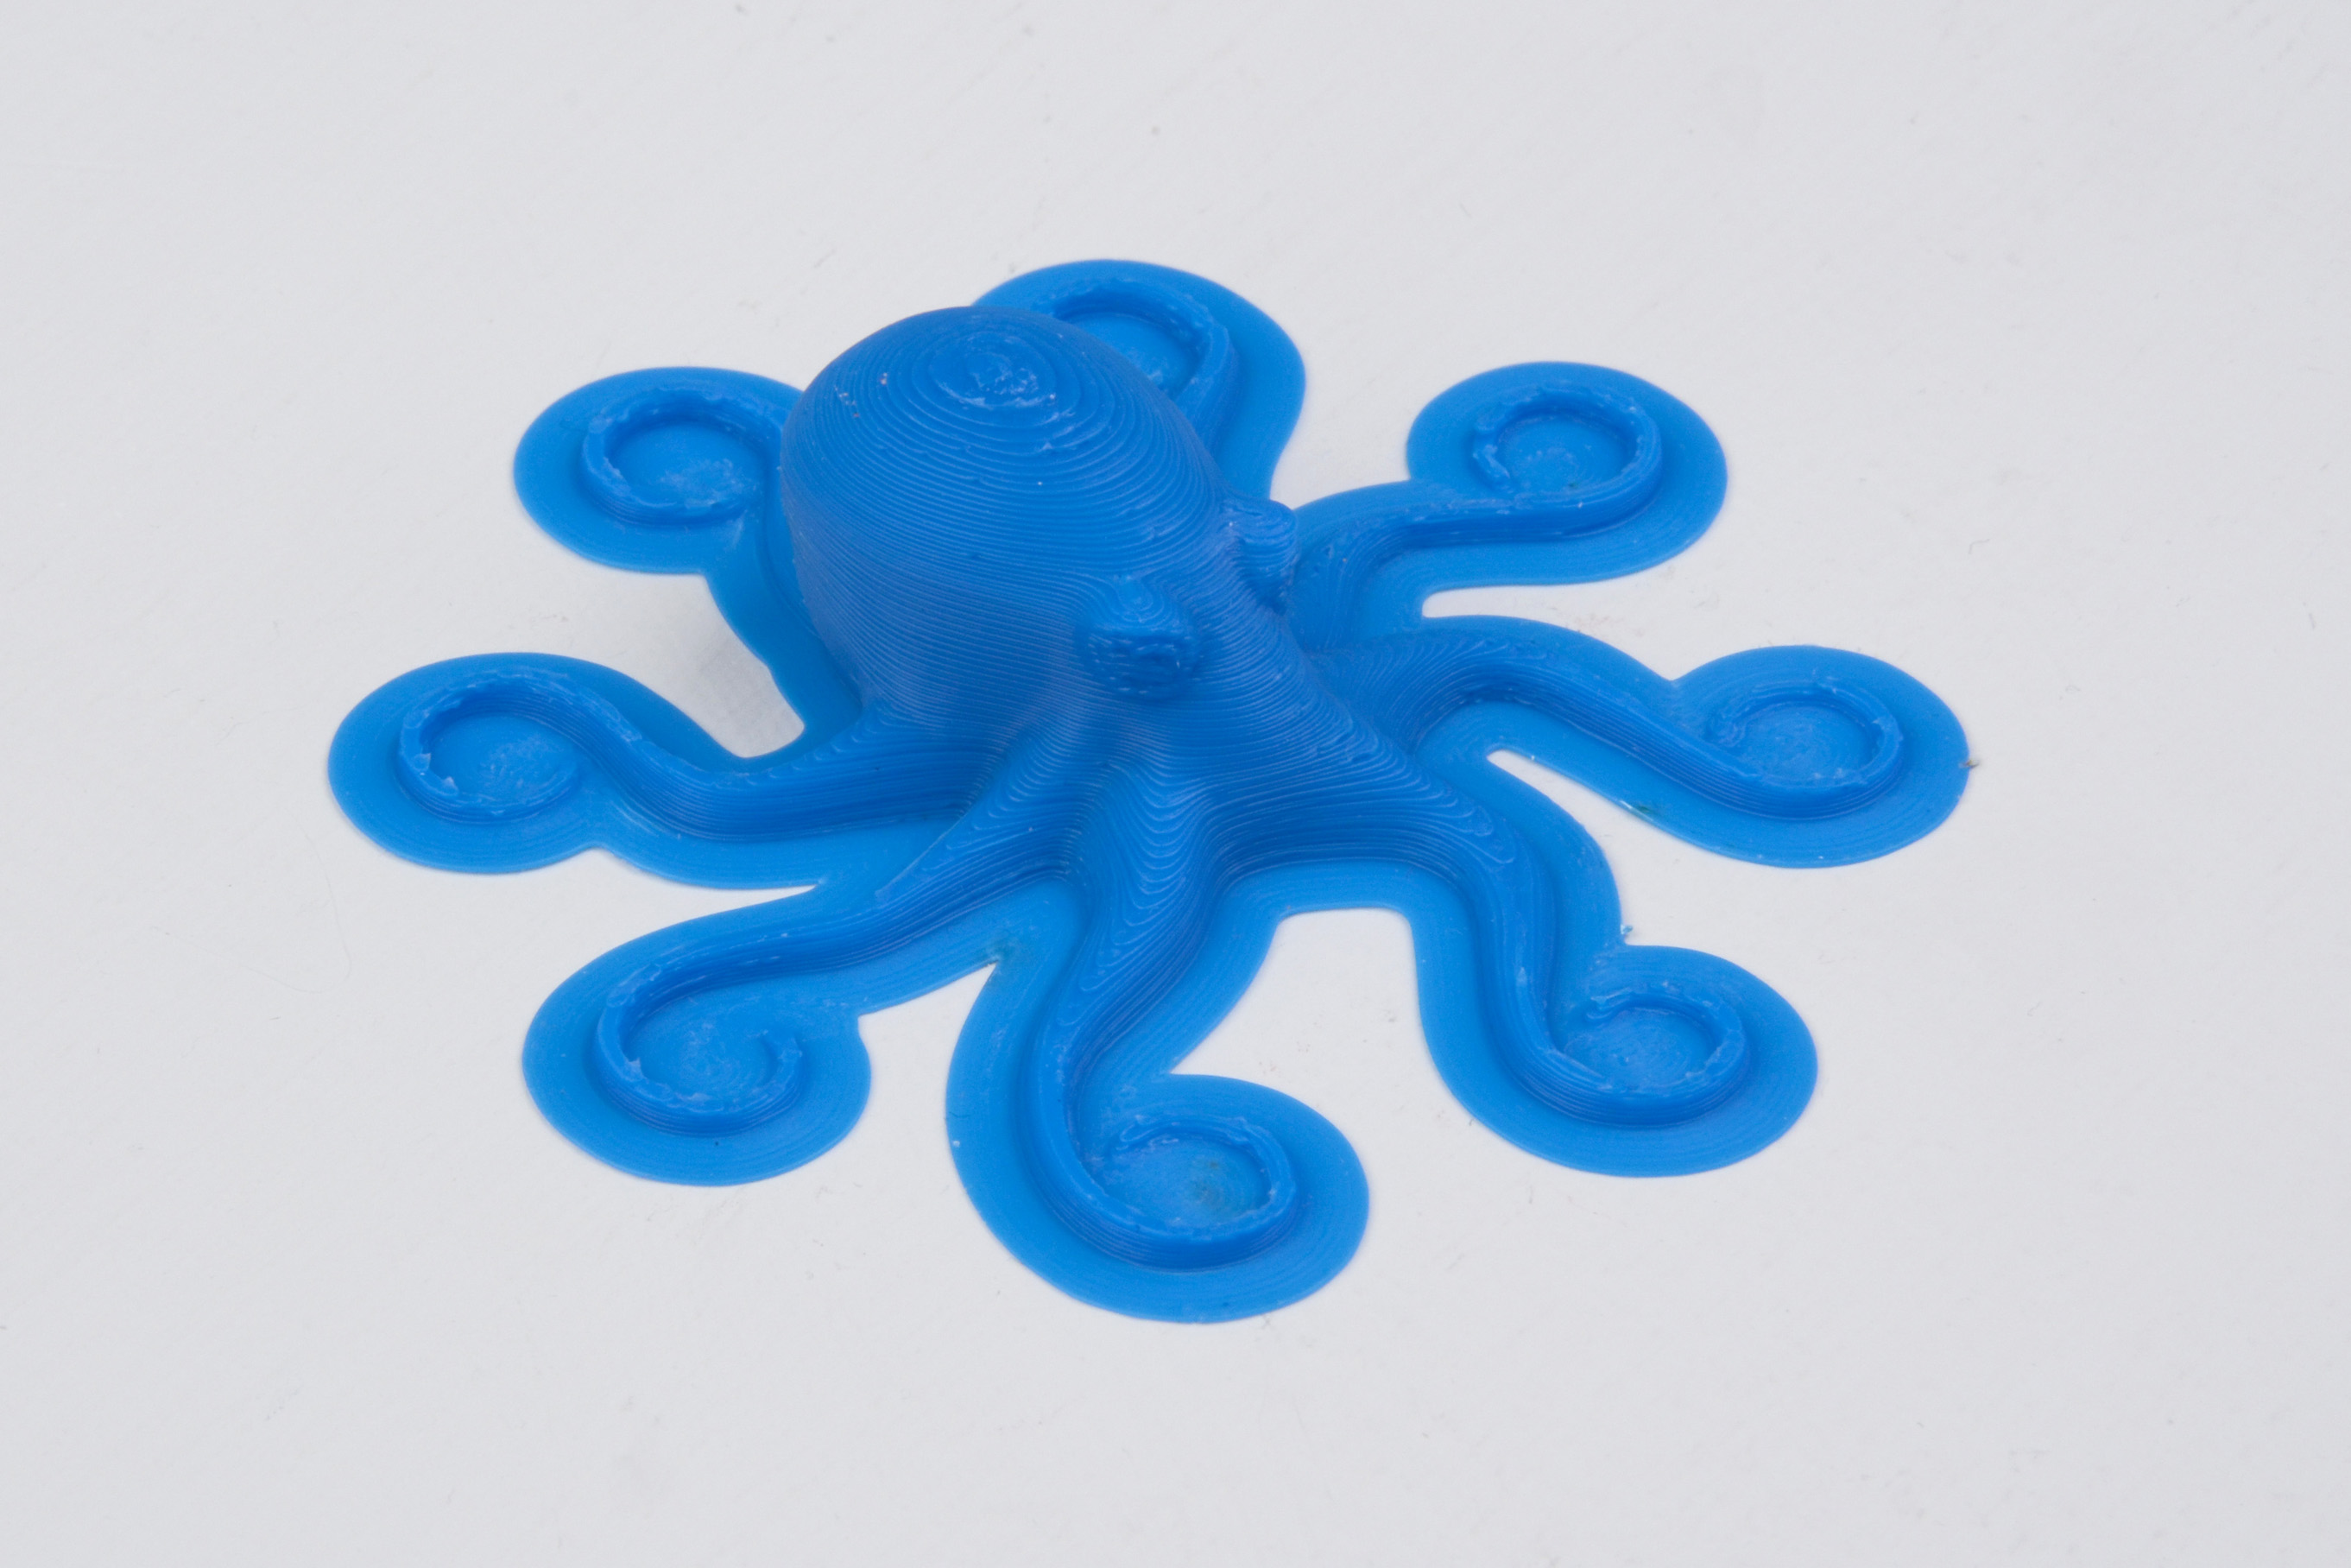
\includegraphics[keepaspectratio=true,width=0.75\textwidth]{simple_mode/brim.jpg}
\caption{Un exemple de bordure.}
\label{fig:an_example_of_brim}
\end{figure}

% paragraph brim (end)

\paragraph{Impression Sequentielle.} % (fold)
\label{par:sequential_printing}
Cette fonction permet de composer un plateau d'objets, en imprimant complétement chaque pièce individuellement, avant de revenir à Z = 0 et de continuer par le suivant. Voir la section sur l'impression séquentielle dans le chapitre des sujets avancés.


\subsection{Paramètres du Filament}
\index{Filament Settings}
\index{Paramètres du Filament}
L'onglet \texttt{Filament Settings} (Paramètres du Filament) sera normalement utilisé peu fréquemment, par exemple lors de la réception d'un nouveau rouleau de filament.

\begin{figure}[H]
\centering
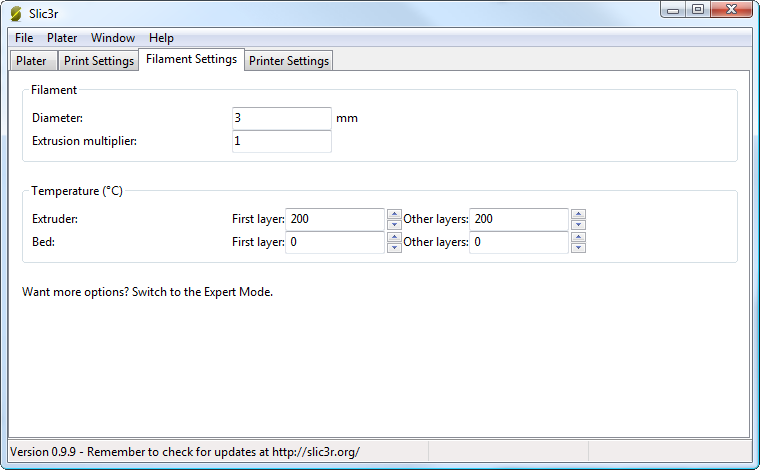
\includegraphics[width=\textwidth]{simple_mode/simple_mode_filament_settings.png}
\caption{Mode Simple: Paramètres du Filament.}
\label{fig:simple_mode_filament_settings}
\end{figure}

\paragraph{Filament.} % (fold)
\label{par:filament}
\index{Filament Settings!Filament}
\index{Paramètres du Filament!Filament}
\index{Filament Settings!Filament!Diameter}
\index{Paramètres du Filament!Filament!Diamètres}
Le paramètre \texttt{Diameter} (Diamètre) aura déjà été rempli à partir de la valeur donnée au cours de l'assistant (voir p.\pageref{sub:4_filament_diameter}), mais peut être modifiée ici.

\index{Filament Settings!Filament!Extrusion multiplier}
\index{Paramètres du Filament!Filament!Multiplicateur d'Extrusion}
La paramètre \texttt{Extrusion multiplier} (Multiplicateur d'Extrusion) permet le réglage fin de la vitesse d'écoulement d'extrusion, et est est donnée en tant que facteur, par exemple, 1 signifie 100 \%, 1,5 signifierait 150 \%. Alors que la valeur devrait idéalement être définie dans le firmware, il peut être utile de tester légères modifications de la vitesse en modifiant cette valeur. Elle modifie la quantité de plastique en proportion et doit être changé par de très petites étapes (par exemple + / - 0,05) car les effets sont très visibles.
% paragraph filament (end)

\paragraph{Température.} % (fold)
\label{par:temperature}
\index{Filament Settings!Temperature!Extruder}
\index{Paramètres du Filament!Température!Extrudeuse}
\index{Filament Settings!Temperature!Bed}
\index{Paramètres du Filament!Température!Lit}
Ces valeurs sont également définies à partir de l'assistant, mais ici la possibilité existe de régler la température de la première couche (voir p.\pageref{sec:the_important_first_layer}).
% paragraph temperature (end)


\subsection{Paramètres de l'Imprimante}
\index{Printer Settings}
\index{Paramètres de l'Imprimante}

Les paramètres de l'imprimante (\texttt{Printer Settings}) ne seront jamais mis à jour, à moins que Slic3r ne soit utilisé pour de nombreuses imprimantes, par exemple, pour une batterie de l'imprimante 3D.

\begin{figure}[H]
\centering
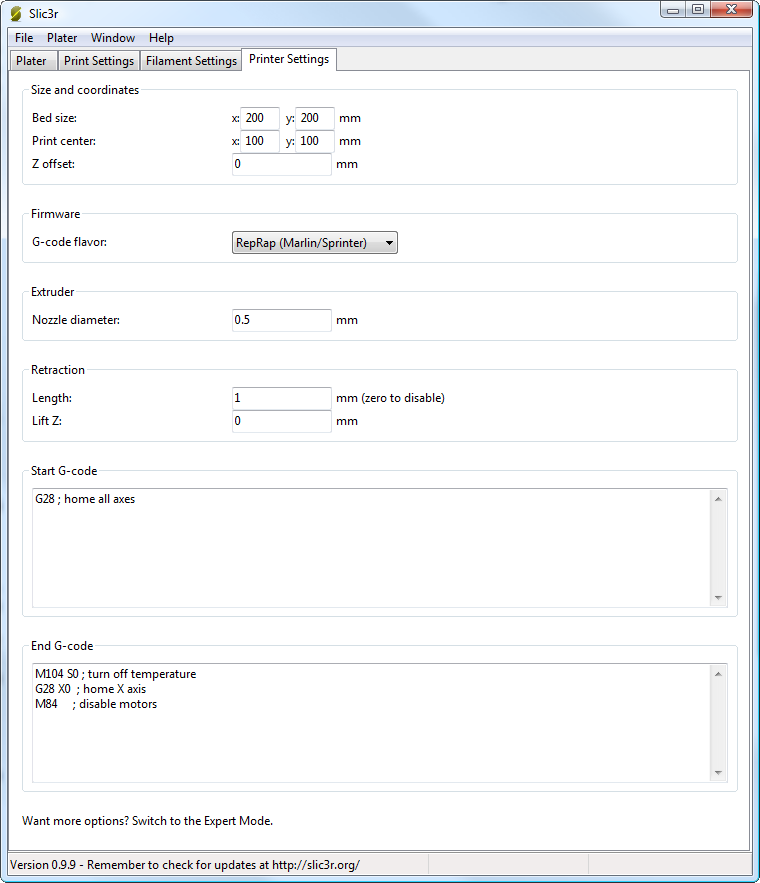
\includegraphics[width=\textwidth]{simple_mode/simple_mode_printer_settings.png}
\caption{Mode Simple: Paramètres de l'Imprimante.}
\label{fig:simple_mode_printer_settings}
\end{figure}

\paragraph{Size and coordinates. (Taille et coordonnées)} % (fold)
\label{par:size_and_coordinates}
\index{Printer Settings!Size and coordinates}
\index{Paramètres de l'Imprimante!Taille et coordonnées}
\index{Printer Settings!Size and coordinates!Bed size}
\index{Paramètres de l'Imprimante!Taille et coordonnées!Taille d lit}
Le paramètre \texttt{Bed size} (Taille du lit) est repris à partir de l'assistant (voir p.\pageref{sub:2_bed_size}) et est utilisé seulement pour la prévisualisation du modèle sur la surface de travail.

\index{Printer Settings!Size and coordinates!Print center}
\index{Paramètres de l'Imprimante!Taille et coordonnées!Centre de l'impression}
Le paramètre \texttt{Print center} (centre de l'impression) defini le point autour duquel l'impression sera centré.  La taille du lit (\texttt{Bed size}) réglée à 200mmx200mm et le centre d'impression (\texttt{Print center}) réglé à 100mmx100mm would placera l'impression au milieu.  Si l'on souhaite imprimer à partir du centre, afin d'eviter des bris sur le rebors du verre, cette option doit être utilisée.

\index{Printer Settings!Size and coordinates!Z offset}
\index{Paramètres de l'Imprimante!Taille et coordonnées!Décalage Z}
\texttt{Z offset} (décalage Z) peut être utilisé pour compenser une fin de course Z mal calibré. Si la buse s'arrête un peu trop loin du lit, on peu conpenser le décalage en ajoutant une valeur négative. La bonne solution est de régler la butée.

La position de fin de course Z optimale est là où la buse touche à peine la surface du lit quand elle se trouve au point d'origine. Une feuille de papier fait un bon indicateur pour cette très petite distance. Il n'est pas recommandé d'utiliser ce paramètre pour essayer d'améliorer l'adhérence couche, en "écrasant" la couche inférieure sur le lit, regardez plutôt les suggestions de la section \ref{sec:the_important_first_layer}.
% paragraph size_and_coordinates (end)

\paragraph{Firmware. (Micrologiciel)} % (fold)
\label{par:firmware}
\index{Printer Settings!Firmware!G-code flavour}
\index{Paramètres de l'Imprimante!Micrologiciel!Variante du G-code}
Comme renseigné par l'assistant (voir p.\pageref{sub:1_firmware_type}), \texttt{G-code flavour} (variante du G-code) définit le dialecte de G-code généré.
% paragraph firmware (end)


\paragraph{Extruder.} % (fold)
\label{par:extruder}
\index{Printer Settings!Extruder!Nozzle diameter}
\index{Paramètres de l'Imprimante!Extrudeuse!Diamètre de la buze}
\texttt{Nozzle diameter} (diamètre dela buze) est renseigné par l'assistant (voir p.\pageref{sub:3_nozzle_diameter}).
% paragraph extruder (end)

\paragraph{Retraction.} % (fold)
\label{par:retraction}
\index{Printer Settings!Extruder!Retraction!Length}
\index{Paramètres de l'Imprimante!Extrudeuse!Rétractation!Longueur}
À moins que le matériau en cours d'extrusion ait une viscosité très élevée, il peut suinter entre extrusions dues à la pesanteur. Cela peut être résolu en rétractant activement le filament entre les extrusions.  Régler le paramètre \texttt{Length} (longueur) à une valeur positive causera le filament à être retiré de plusieurs millimètres avant le déplacement. Le retrait sera alors compensée par la même quantité après le déménagement de Voyage, avant de commencer le nouveau chemin d'extrusion.

Une valeur comprise entre 1 et 2 mm est habituellement recommandé. Extrudeuses sous gaine peuvent avoir besoin de 4 ou 5 mm en raison de l'hystérésis introduit par le tube.
\index{Printer Settings!Extruder!Retraction!Lift Z}
\index{Paramètres de l'Imprimante!Extrudeuse!Rétractation!élévation Z}
Régler le paramètre \texttt{Lift Z} (Elévation Z) à une valeur positive relèvera l'extrudeuse sur l'axe Z de ce nombre de millimètres durant chaque déplacement. Cela peut être utile pour s'assurer que la buse n'accroche pas la couche précedente, mais cette valeur n'est généralement pas nécessaire et ralentit la vitesse d'impression. Une valeur de 0,1 mm est généralement suffisante.
% paragraph retraction (end)

\paragraph{Start, End and Layer Chance G-codes.} % (fold)
\label{par:start_end_g_code}
\index{Printer Settings!Custom G-code!Start G-code}
\index{Paramètres de l'Imprimante!G-code personalisé!G-code de démarrage}
\index{Printer Settings!Custom G-code!End G-code}
\index{Paramètres de l'Imprimante!G-code personalisé!G-code de fin}
Les commandes G-code personnalisées peuvent être exécutés avant que l'impression démarre et après la fin de l'impression.

Des variables d'environements peuvent être insérés dans les commandes G-code\footnote{https://github.com/alexrj/Slic3r/wiki/FAQ\#what-placeholders-can-i-use-in-custom-g-code}.  Par exemple [next\_extruder] retournerait l'index de la prochaine extrudeuse.

Le wiki RepRap est une bonne ressource pour en apprendre davantage sur la variété de G-codes disponibles: \texttt{http://reprap.org/wiki/G-code}.

Remarque: Assurez-vous de vérifier qu'un G-code utilisé est valide pour votre micrologiciel.

Les commandes saisies dans la section \texttt{Start G-code} (G-code de démarrage) 
sont insérés au début du fichier de sortie, directement après les instructions de commande de température de l'extrudeuse et du lit. Notez que si les commandes de contrôle de la température sont spécifiés (M104 et M190), alors celles-ci remplaceront les températures G-codes introduites par les paramètres \texttt{Filament}.

Les G-codes courant à utiliser avant le début d'impression sont:
\begin{itemize}
	\item \textbf{G28}  - Placer chaques axes à sa position d'origine.
\end{itemize}


Les G-codes courants à utiliser aprés la fin de l'impression sont:
\begin{itemize}
	\item \textbf{M104 S0}  - Règle la température de l'extrudeuse à zéro.
	\item \textbf{M140 S0} - Définit la température du lit chauffant à zéro.
	\item \textbf{G28 X0} - Place l'axe X à son origine.
	\item \textbf{M84}  - Désactive les moteurs.
\end{itemize}
% paragraph start_end_g_code (end)

% section simple_mode (end)\section{Simple Mode}
